\documentclass[english]{SPFShortReport}
\usepackage{subfigure}
\usepackage{spfFigures}
\usepackage{longtable}
\usepackage{url}
\usepackage{gensymb}
\usepackage[yyyymmdd,hhmmss]{datetime}
\reportName{Type977 fitting for heat pump SIN-26TU}
\reportSubName{Parametric Heat Pump calculation} 
\reportDate{\today \hspace{0.1cm} at: \currenttime \hspace{0.1cm} h} 
\author{Dani Carbonell}
\address{dani.carbonell@spf.ch}
\begin{document}
\begin{table}[!ht]
\begin{small}
\caption{Fitted coefficients for the heat pump.}
\begin{center}
\resizebox{12cm}{!} 
{
\begin{tabular}{l | c c } 
\hline
\hline
Coefficient &Description & \\ 
 & &$[kW]$\\ 
\hline
$P_{Q_{1}}$ & \emph{$1^{st}$ condenser polynomial coefficient}  & 2.5644e+01    \\ 
$P_{Q_{2}}$ & \emph{$2^{st}$ condenser polynomial coefficient}  & 3.0014e+02    \\ 
$P_{Q_{3}}$ & \emph{$3^{st}$ condenser polynomial coefficient}  & 5.9163e+01    \\ 
$P_{Q_{4}}$ & \emph{$4^{st}$ condenser polynomial coefficient}  & -5.9720e+02    \\ 
$P_{Q_{5}}$ & \emph{$5^{st}$ condenser polynomial coefficient}  & 5.1391e+02    \\ 
$P_{Q_{6}}$ & \emph{$6^{st}$ condenser polynomial coefficient}  & -2.9866e+02    \\ 
\hline
$P_{COP_{1}}$ & \emph{$1^{st}$ COP polynomial coefficient}  & 6.7660e+00    \\ 
$P_{COP_{2}}$ & \emph{$2^{st}$ COP polynomial coefficient}  & 7.0047e+01    \\ 
$P_{COP_{3}}$ & \emph{$3^{st}$ COP polynomial coefficient}  & -5.1288e+00    \\ 
$P_{COP_{4}}$ & \emph{$4^{st}$ COP polynomial coefficient}  & -2.9395e+02    \\ 
$P_{COP_{5}}$ & \emph{$5^{st}$ COP polynomial coefficient}  & 1.0724e+02    \\ 
$P_{COP_{6}}$ & \emph{$6^{st}$ COP polynomial coefficient}  & -7.2713e+01    \\ 
\hline
$\dot m_{cond}$ & 4500.00 $[kg/h]$ \\ 
$\dot m_{evap}$ & 4500.00 $[kg/h]$ \\ 
\hline
$COP_{nom}$ (A0W35)& 4.81 \\ 
$Q_{cond,nom}$ (A0W35)& 26.40 $[kW]$\\ 
$Q_{evap,nom}$ (A0W35)& 20.92 $[kW]$\\ 
$W_{comp,nom}$ (A0W35)& 5.48 $[kW]$\\ 
\hline
 $RMS_{COP}$ & $7.10e-02$ \\ 
 $RMS_{Q_{cond}}$ & $2.00e-01$ \\ 
 $RMS_{W_{comp}}$ & $8.30e-02$ \\ 
\hline
Fit model & Average Temperature\\ 
\hline
\hline
\end{tabular}
}
\label{CoefTable}
\end{center}
\end{small}
\end{table}
\begin{table}[!ht]
\begin{small}
\caption{Differences between experiments and fitted data for the heat pump.          $error=100 \cdot |\frac{Q_{exp}-Q_{num}}{Q_{exp}}|$ and $RMS = \sqrt { \sum{\frac{(Q_{exp}-Q_{num})^2}{n_p}} }$ where $n_p$ is the number of data points.}
\begin{center}
\resizebox{12cm}{!} 
{
\begin{tabular}{l | c c c c c c c c c c } 
\hline
\hline
$T_{cond,out}$ &$T_{evap,in}$ &$COP$ &$COP_{exp}$ &error &$Q_{cond}$ &$Q_{cond,exp}$ &error &$W_{comp}$ &$W_{comp,exp}$ &error \\ 
$^oC$ &$^oC$ &$[-]$ &$[-]$ &$[\%]$ &$[kW]$ &$[kW]$ &$[\%]$ &$[kW]$ &$[kW]$ &$[\%]$\\ 
\hline
35.00  & -5.00 & 4.30 & 4.40 & 2.2 & 23.03 & 23.40 & 1.6 & 5.36 & 5.32 & 0.66\\ 
35.00  & 0.00 & 4.85 & 4.70 & 3.0 & 26.63 & 26.20 & 1.6 & 5.50 & 5.57 & 1.34\\ 
35.00  & 5.00 & 5.48 & 5.46 & 0.4 & 30.52 & 30.50 & 0.1 & 5.57 & 5.59 & 0.34\\ 
50.00  & -5.00 & 3.25 & 3.21 & 1.3 & 22.40 & 22.40 & 0.0 & 6.90 & 6.99 & 1.30\\ 
50.00  & 0.00 & 3.54 & 3.43 & 3.0 & 25.53 & 25.27 & 1.0 & 7.22 & 7.36 & 1.94\\ 
50.00  & 5.00 & 3.91 & 3.88 & 0.7 & 28.97 & 29.03 & 0.2 & 7.41 & 7.48 & 0.93\\ 
45.00  & -5.00 & 3.65 & 3.72 & 1.9 & 22.80 & 22.90 & 0.4 & 6.25 & 6.15 & 1.51\\ 
45.00  & 0.00 & 4.02 & 3.98 & 1.1 & 26.08 & 25.73 & 1.4 & 6.48 & 6.47 & 0.23\\ 
45.00  & 5.00 & 4.49 & 4.56 & 1.5 & 29.67 & 29.77 & 0.3 & 6.61 & 6.54 & 1.22\\ 
55.00  & 0.00 & 3.00 & 3.00 & 0.2 & 24.80 & 24.80 & 0.0 & 8.27 & 8.26 & 0.18\\ 
55.00  & 5.00 & 3.28 & 3.36 & 2.3 & 28.10 & 28.30 & 0.7 & 8.56 & 8.43 & 1.60\\ 
35.00  & 10.00 & 6.18 & 6.20 & 0.4 & 34.70 & 34.80 & 0.3 & 5.62 & 5.61 & 0.10\\ 
35.00  & 15.00 & 6.95 & 6.94 & 0.0 & 39.16 & 39.10 & 0.1 & 5.64 & 5.63 & 0.14\\ 
50.00  & 10.00 & 4.35 & 4.32 & 0.8 & 32.70 & 32.80 & 0.3 & 7.51 & 7.60 & 1.10\\ 
50.00  & 15.00 & 4.86 & 4.74 & 2.5 & 36.71 & 36.57 & 0.4 & 7.55 & 7.71 & 2.09\\ 
45.00  & 10.00 & 5.02 & 5.12 & 2.0 & 33.56 & 33.80 & 0.7 & 6.69 & 6.60 & 1.28\\ 
45.00  & 15.00 & 5.62 & 5.67 & 0.9 & 37.72 & 37.83 & 0.3 & 6.72 & 6.67 & 0.66\\ 
55.00  & 10.00 & 3.64 & 3.70 & 1.8 & 31.68 & 31.80 & 0.4 & 8.71 & 8.59 & 1.41\\ 
55.00  & 15.00 & 4.06 & 4.03 & 0.6 & 35.53 & 35.30 & 0.7 & 8.76 & 8.76 & 0.08\\ 
\hline 
 Sum &  & &  & 26.8 &  &  & 10.6 & &  & 18.09\\ 
\hline 
 $RMS_{COP}$ & $7.10e-02$ \\ 
 $RMS_{Q_{cond}}$ & $2.00e-01$ \\ 
 $RMS_{W_{comp}}$ & $8.30e-02$ \\ 
\hline
\hline
\end{tabular}
}
\label{ErrorsTable}
\end{center}
\end{small}
\end{table}
\begin{figure}[!ht]
\begin{center}
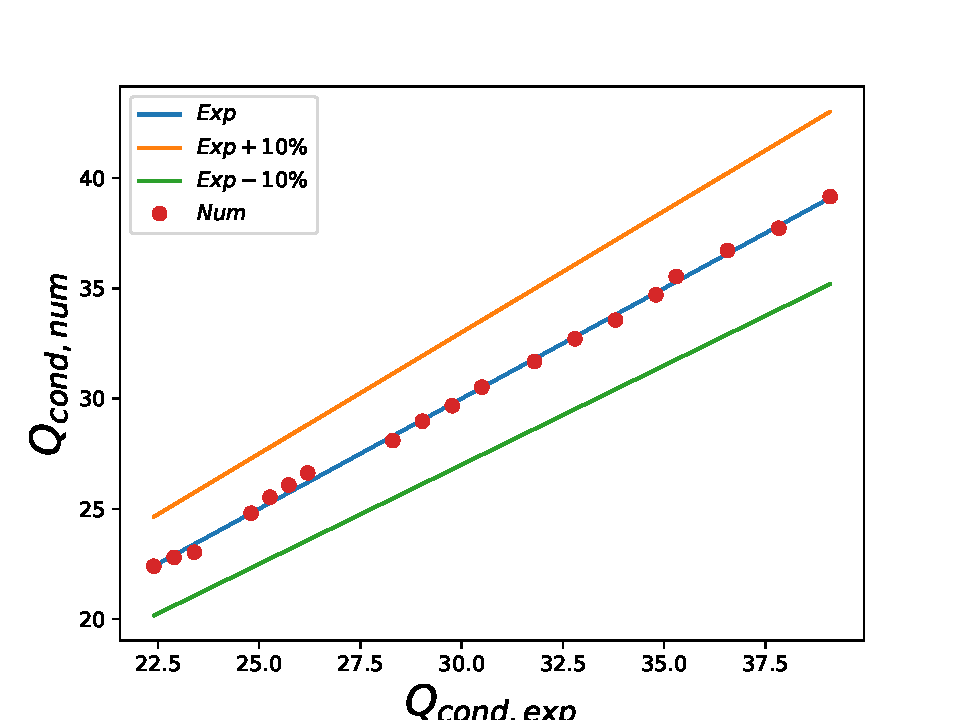
\includegraphics[width=1\textwidth]{C:/Daten/spfPackages/GIT/spfTrnsysFiles/HeatPump/BrineToWater/Walter Meier/SIN-26TU/SIN-26TU-Qcond.pdf}
\caption{$Q_{cond}$ differences between experiments and fitted data}
\label{QcongFig}
\end{center}
\end{figure}
\begin{figure}[!ht]
\begin{center}
\includegraphics[width=1\textwidth]{C:/Daten/spfPackages/GIT/spfTrnsysFiles/HeatPump/BrineToWater/Walter Meier/SIN-26TU/SIN-26TU-Qcomp.pdf}
\caption{$W_{comp}$ differences between experiments and fitted data}
\label{QcompFig}
\end{center}
\end{figure}
\begin{figure}[!ht]
\begin{center}
\includegraphics[width=1\textwidth]{C:/Daten/spfPackages/GIT/spfTrnsysFiles/HeatPump/BrineToWater/Walter Meier/SIN-26TU/SIN-26TU-COP.pdf}
\caption{$COP$ differences between experiments and fitted data}
\label{COPFig}
\end{center}
\end{figure}
\end{document}
